\documentclass{ximera}

\input{../preamble.tex}

\outcome{Know the properties of rational functions.}
\outcome{Understand the definition of a rational function.}

\title[Dig-In:]{Rational equations and inequalities}


\begin{document}
\begin{abstract}
 Equations and inequalities with Rational Functions
\end{abstract}
\maketitle


\section{Rational equations and inequalities}
To solve equations involving rational expressions, we have the freedom to clear out fractions before proceeding.
After multiplying both sides by the common denominator, we are left with a polynomial equation.
\begin{example}
	Solve the equation
	\[  \frac{2}{x} + \frac{3x}{x+1} = 4.\]
	\begin{explanation}
		The common denominator is $x(x+1)$.  We multiply both sides by $x(x+1)$ to clear out the fractions.
		\begin{align*}
			\frac{2}{x} + \frac{3x}{x+1} &= 4	\\
			x(x+1) \left( \frac{2}{x} + \frac{3x}{x+1} \right) &= x(x+1) ( 4 )\\
			x(x+1) \cdot \frac{2}{x}  + x(x+1) \cdot \frac{3x}{x+1} &= 4x(x+1)\\
			2(x+1) + 3x(x) &= 4x^2 + 4x\\
			3x^2 + 2x + 2 &= 4x^2 + 4x\\
			x^2 + 2x - 2 &= 0.
		\end{align*}
		The quadratic formula gives solutions as $\displaystyle x = \dfrac{-2 \pm \sqrt{12}}{2} = -1 \pm \sqrt{3}$.
		
		If we look back at the original equation, we notice that there are some numbers that we are not allowed to plug in for $x$.  When $x=0$ or $x=-1$,
		the left-hand side of the equation is not defined due to a division by zero issue.  Since neither $-1 + \sqrt{3}$ nor $-1-\sqrt{3}$ have such an issue,
		they are both solutions.
	\end{explanation}
\end{example}

\begin{question}
	One solution of the equation \[ \dfrac{2}{x+1}+ \dfrac{1}{x+2} = 1 \] is $x = \sqrt{3}$.  Find another solution. 
	\begin{prompt}
		\[ x = \answer{-\sqrt{3}} \]
	\end{prompt}
\end{question}

\section{Inequalities}
When faced with nonlinear inequalities, such as those involving general rational functions, we make use of a sign chart.
The inequality in the following example is not given in factored form, so we have some work to do.
\begin{example}
	Solve the inequality $\displaystyle x^2 + 5x \leq -10 -\dfrac{16}{x-2}$.
	\begin{explanation}
		We'll begin by moving everything to one side, then combining them all together into a single fraction.
		\begin{align*}
			x^2 + 5x &\leq -10 -\dfrac{16}{x-2}\\
			x^2 + 5x +10 +\dfrac{16}{x-2} &\leq 0\\
			\left(x^2+5x+10\right) \cdot \left(\dfrac{x-2}{x-2}\right) +\dfrac{16}{x-2} &\leq 0\\
			\dfrac{x^3+3x^2-20}{x-2} + \dfrac{16}{x-2} &\leq 0\\
			\dfrac{x^3+3x^2-4}{x-2} &\leq 0\\
			\dfrac{(x-1)(x+2)^2}{x-2} &\leq 0
		\end{align*}
		Now that the inequality is in a better form for us to work with, we'll build a sign chart like we did in the last example.

		\begin{tikzpicture} 
			\tkzTabInit[lgt=2,espcl=1] 
				{$x$         /1, 
				$x-1$   /1, 
				$\left(x+2\right)^2$  /1,
				$x-2$       /1}% 
				{  , $-2$ , $1$ ,$2$,  }% 
			\tkzTabLine{ , - , t , - , t , + , d , + ,}
			\tkzTabLine{ , + , t , + , t , + , d , + ,}
			\tkzTabLine{ , - , t , - , t , - , d , +, }
		\end{tikzpicture} 

		We see from the chart that $\displaystyle \dfrac{(x-1)(x+2)^2}{x-2}$ will be negative in $(1,2)$.  At $x=-2$ and $x=1$ it is zero.
		The solution is then: $\left\{ -2\right\} \cup [ 1, 2 )$.
	\end{explanation}
\end{example}


\begin{problem}
	Find the solution of the inequality: $\displaystyle x + \dfrac{9}{x-1} > 5$.
	\begin{multipleChoice}
		\choice{$(1, \infty)$}
		\choice{$[1,\infty)$}
		\choice[correct]{$(1,2)\cup (2,\infty)$}
		\choice{$\{1\} \cup [2,\infty)$}
		\choice{none of the above}
	\end{multipleChoice}
\end{problem}


\begin{example}
	Solve the inequality
	\[ \frac{1}{x-2} - \frac{4}{x+1} \leq 3 \]
	\begin{explanation}
		We'll start by moving everything to the left-hand side and combining them into a single fraction.
		\begin{align*}
			\frac{1}{x-2} - \frac{4}{x+1} &\leq 3 \\
			\frac{1}{x-2} - \frac{4}{x+1} - 3 &\leq 0\\
			\frac{1(x+1)}{(x-2)(x+1)} - \frac{4(x-2)}{(x+1)(x-2)} - \frac{3(x+1)(x-2)}{(x+1)(x-2)} &\leq 0\\
			\frac{(x+1) - (4x-8) - (3x^2-3x-6)}{(x+1)(x-2)} &\leq 0\\
			\frac{-3x^2+15}{(x+1)(x-2)} &\leq 0\\
			\frac{-3(x^2-5)}{(x+1)(x-2)} &\leq 0
		\end{align*}
		To solve this, we'll construct a sign chart.  We start by noticing that $x^2-5 =0$ only if $x = \pm \sqrt{5}$.
		\begin{tikzpicture} 
			\tkzTabInit[lgt=2,espcl=1] 
				{$x$         /1, 
				$-3$    /1,
				$x^2-5$   /1, 
				$x+1$  /1,
				$x-2$       /1}% 
				{  , $-\sqrt{5}$ , $-1$ , $2$, $\sqrt{5}$,   }% 
			\tkzTabLine{ , - , t , - , d , - , d , - , t, -, }
			\tkzTabLine{ , + , t , - , d , - , d , - , t, +,}
			\tkzTabLine{ , - , t , - , d , + , d , +, t, +, }
			\tkzTabLine{ , - , t , - , d , - , d , +, t, +, }
		\end{tikzpicture} 
		
		We see from the sign chart, that the solution is $\displaystyle \left( -\infty, -\sqrt{5} \right] \bigcup \left(-1, 2\right) \bigcup \left[ \sqrt{5}, \infty \right)$.
	\end{explanation}
\end{example}







\end{document}
